\documentclass{aa}
\usepackage{graphicx}
\usepackage{booktabs}
\usepackage{txfonts}
\usepackage{xcolor}
\definecolor{linkblue}{RGB}{25,70,110}
\usepackage[colorlinks=true,allcolors=linkblue]{hyperref}
\graphicspath{{figures/}}
\newcommand{\px}{\,\mathrm{px}}

\begin{document}
\title{Blind astrometry and instrumental photometry of wide-field sky images}
\subtitle{From single fisheye photographs to repeated native-colour FITS observations}
\author{P. Thejll\inst{1}\corrauth{pth@dmi.dk}}
\institute{Danish Meteorological Institute, Skt. Kjelds Plads 11,
  DK-2100 Copenhagen~\O, Denmark}
\date{Received 18 September 2026 / Accepted ---}

\abstract
{Wide-field images preserve stellar positions, colour-dependent fluxes,
atmospheric extinction, and sometimes planetary configurations even when their
metadata or calibration are incomplete. Extracting these signals together
requires a solver that tolerates severe optical distortion, uncertain parity,
saturation, and crowded fields.}
{We present and test a reproducible workflow for blind astrometric calibration
and instrumental photometry of circular-fisheye and other very wide-field
images. We also test which secondary constraints---photometric zenith,
catalogue epoch, and planetary ephemerides---are identifiable from the pixels.}
{Sources are detected without withholding bright or saturated objects. A
lost-in-space stellar bootstrap is refined with the eight-parameter Barghini
camera model, angular sky association, and robust fitting. Native red, green,
and blue FITS planes are measured independently; repeated exposures are linked
through catalogue identity to form differential light curves.}
{A dense Milky Way photograph yields 3653 stellar associations with
0.398-pixel RMS residual. A representative three-plane MMTO exposure yields
1385 fitted stars with 0.338-pixel (2.61-arcmin) RMS residual; Jupiter is
recovered after the stellar fit at 0.218 pixels despite saturation, using
unsaturated wing pixels. Across 65 MMTO exposures, 86\,271 quality-controlled
measurements form 162 repeated stellar series. A separate fisheye photograph
shows that a planetary configuration can select the correct calendar date,
although the site-supplied timing minimum is uncertain by several hours.}
{A single model can support astrometry, photometry, and post-fit solar-system
validation across heterogeneous wide fields, but not every image contains
every constraint. Archives that retain native-colour FITS planes and repeated
observations are therefore substantially more valuable than rendered previews:
they preserve detector-level information for saturation recovery, colour
diagnostics, extinction tests, and time-series photometry.}
\keywords{astrometry -- methods: data analysis -- techniques: image processing
-- techniques: photometric -- atmospheric effects -- surveys}
\maketitle

\section{Introduction}
\label{sec:introduction}

All-sky and very wide-field cameras record more than a view of the sky. Their
pixels can contain a stellar coordinate system, colour-dependent instrumental
fluxes, atmospheric gradients, and moving solar-system objects. These signals
are useful for monitoring transparency, cloud, night-sky brightness, meteors,
and variable stars, and can also validate image time and provenance. The
difficulty is that a wide field is not well described by a tangent plane.
Strong radial distortion, imperfect centring, parity ambiguity, horizon
structure, crowding, and saturation must all be handled without moving
measured centroids to make a fit appear better.

Blind methods establish a coordinate system without a supplied pointing
\citep{Lang2010}. Dedicated calibrations describe large radial and azimuthal
departures from simpler projections
\citep{borovicka1995,Barghini2019,Jeanne2019}. Recent applications demonstrate
the scientific use of calibrated all-sky cameras \citep{Hung2024,Yin2025} and
explicit models for super-wide fields \citep{AntunaSanchez2022,Yang2025}.
Here we join blind initialization, dense association, robust global refinement,
and native-plane photometry in one inspectable workflow.

The primary contract is strict. Site, time, camera, and object names do not seed
the stellar solution. Every detected source remains available, including large
and saturated detections. Metadata may be revealed only after astrometric
parameters are fixed, for separate validation. A planet matched at a FITS
timestamp is therefore a post-fit validation; a topocentric date search with a
supplied site is conditional rather than fully blind epoch inference.

We test heterogeneous single images and a repeated native-colour archive from
the Mountain Meteorological Test Observatory (MMTO). Stellar catalogue epoch
and photometric zenith are reported only when identifiable. The result is not
that every image yields every quantity, but that original planes and repeated
exposures preserve a much wider set of defensible measurements.

\section{Image and catalogue data}
\label{sec:data}

The test image is \emph{Southern Milky Way and Planets}, photographed at
Atacama Lodge near San Pedro de Atacama, Chile. The publisher states 2018 April
15 at 06:55 UTC, a Nikon D750, a Sigma 8-mm circular fisheye, and one 240-s
exposure at $f/4.5$ and ISO 1600 \citep{Espenak2018}. The published original is
$4016\times4016$ pixels; we analysed the available $925\times925$-pixel JPEG.
The file metadata likewise report a Nikon D750, 8.0-mm focal length, 240 s,
$f/4.5$, and ISO 1600. Its lens-model field instead gives 8.0 mm at $f/3.5$;
we retain this discrepancy as metadata rather than using either lens label as a
fit constraint.

We used a fixed local copy of the Tycho-2 catalogue \citep{Hog2000}, augmented
by bright Hipparcos stars where required. Catalogue coordinates with two
proper-motion components were propagated to the candidate epoch. A scan of the
stellar residual against catalogue reference year was also made as a check on
whether proper motion alone dated this recent image.


The broader tests include a dense circular-fisheye Milky Way photograph,
APICAM and Subaru images at different source densities and plate scales, and a
sequence of three-plane MMTO FITS files. One representative MMTO exposure, at
the archive timestamp 2026 January 17 01:43:54, contains three
$1411\times1422$ planes and a 20-s integration. These are numerical red, green,
and blue detector measurements, not a rendered colour preview.

The historical examples use Tycho-2 and bright Hipparcos stars; the denser
workflow uses Gaia DR3 astrometry where appropriate \citep{GaiaDR3}.
Planet positions are calculated independently of source names using standard
ephemerides and topocentric transformations
\citep{Simon1994,Giorgini1996,Astropy2022}. FITS is central to the photometric
work because it retains numerical detector planes, headers, and dynamic range
in a standard astronomical container \citep{Pence2010}. The Espenak site is
supplied to its topocentric calculation, so that example tests calendar-date
recovery conditional on location rather than blind recovery of place and time.
\begin{figure*}
  \centering
  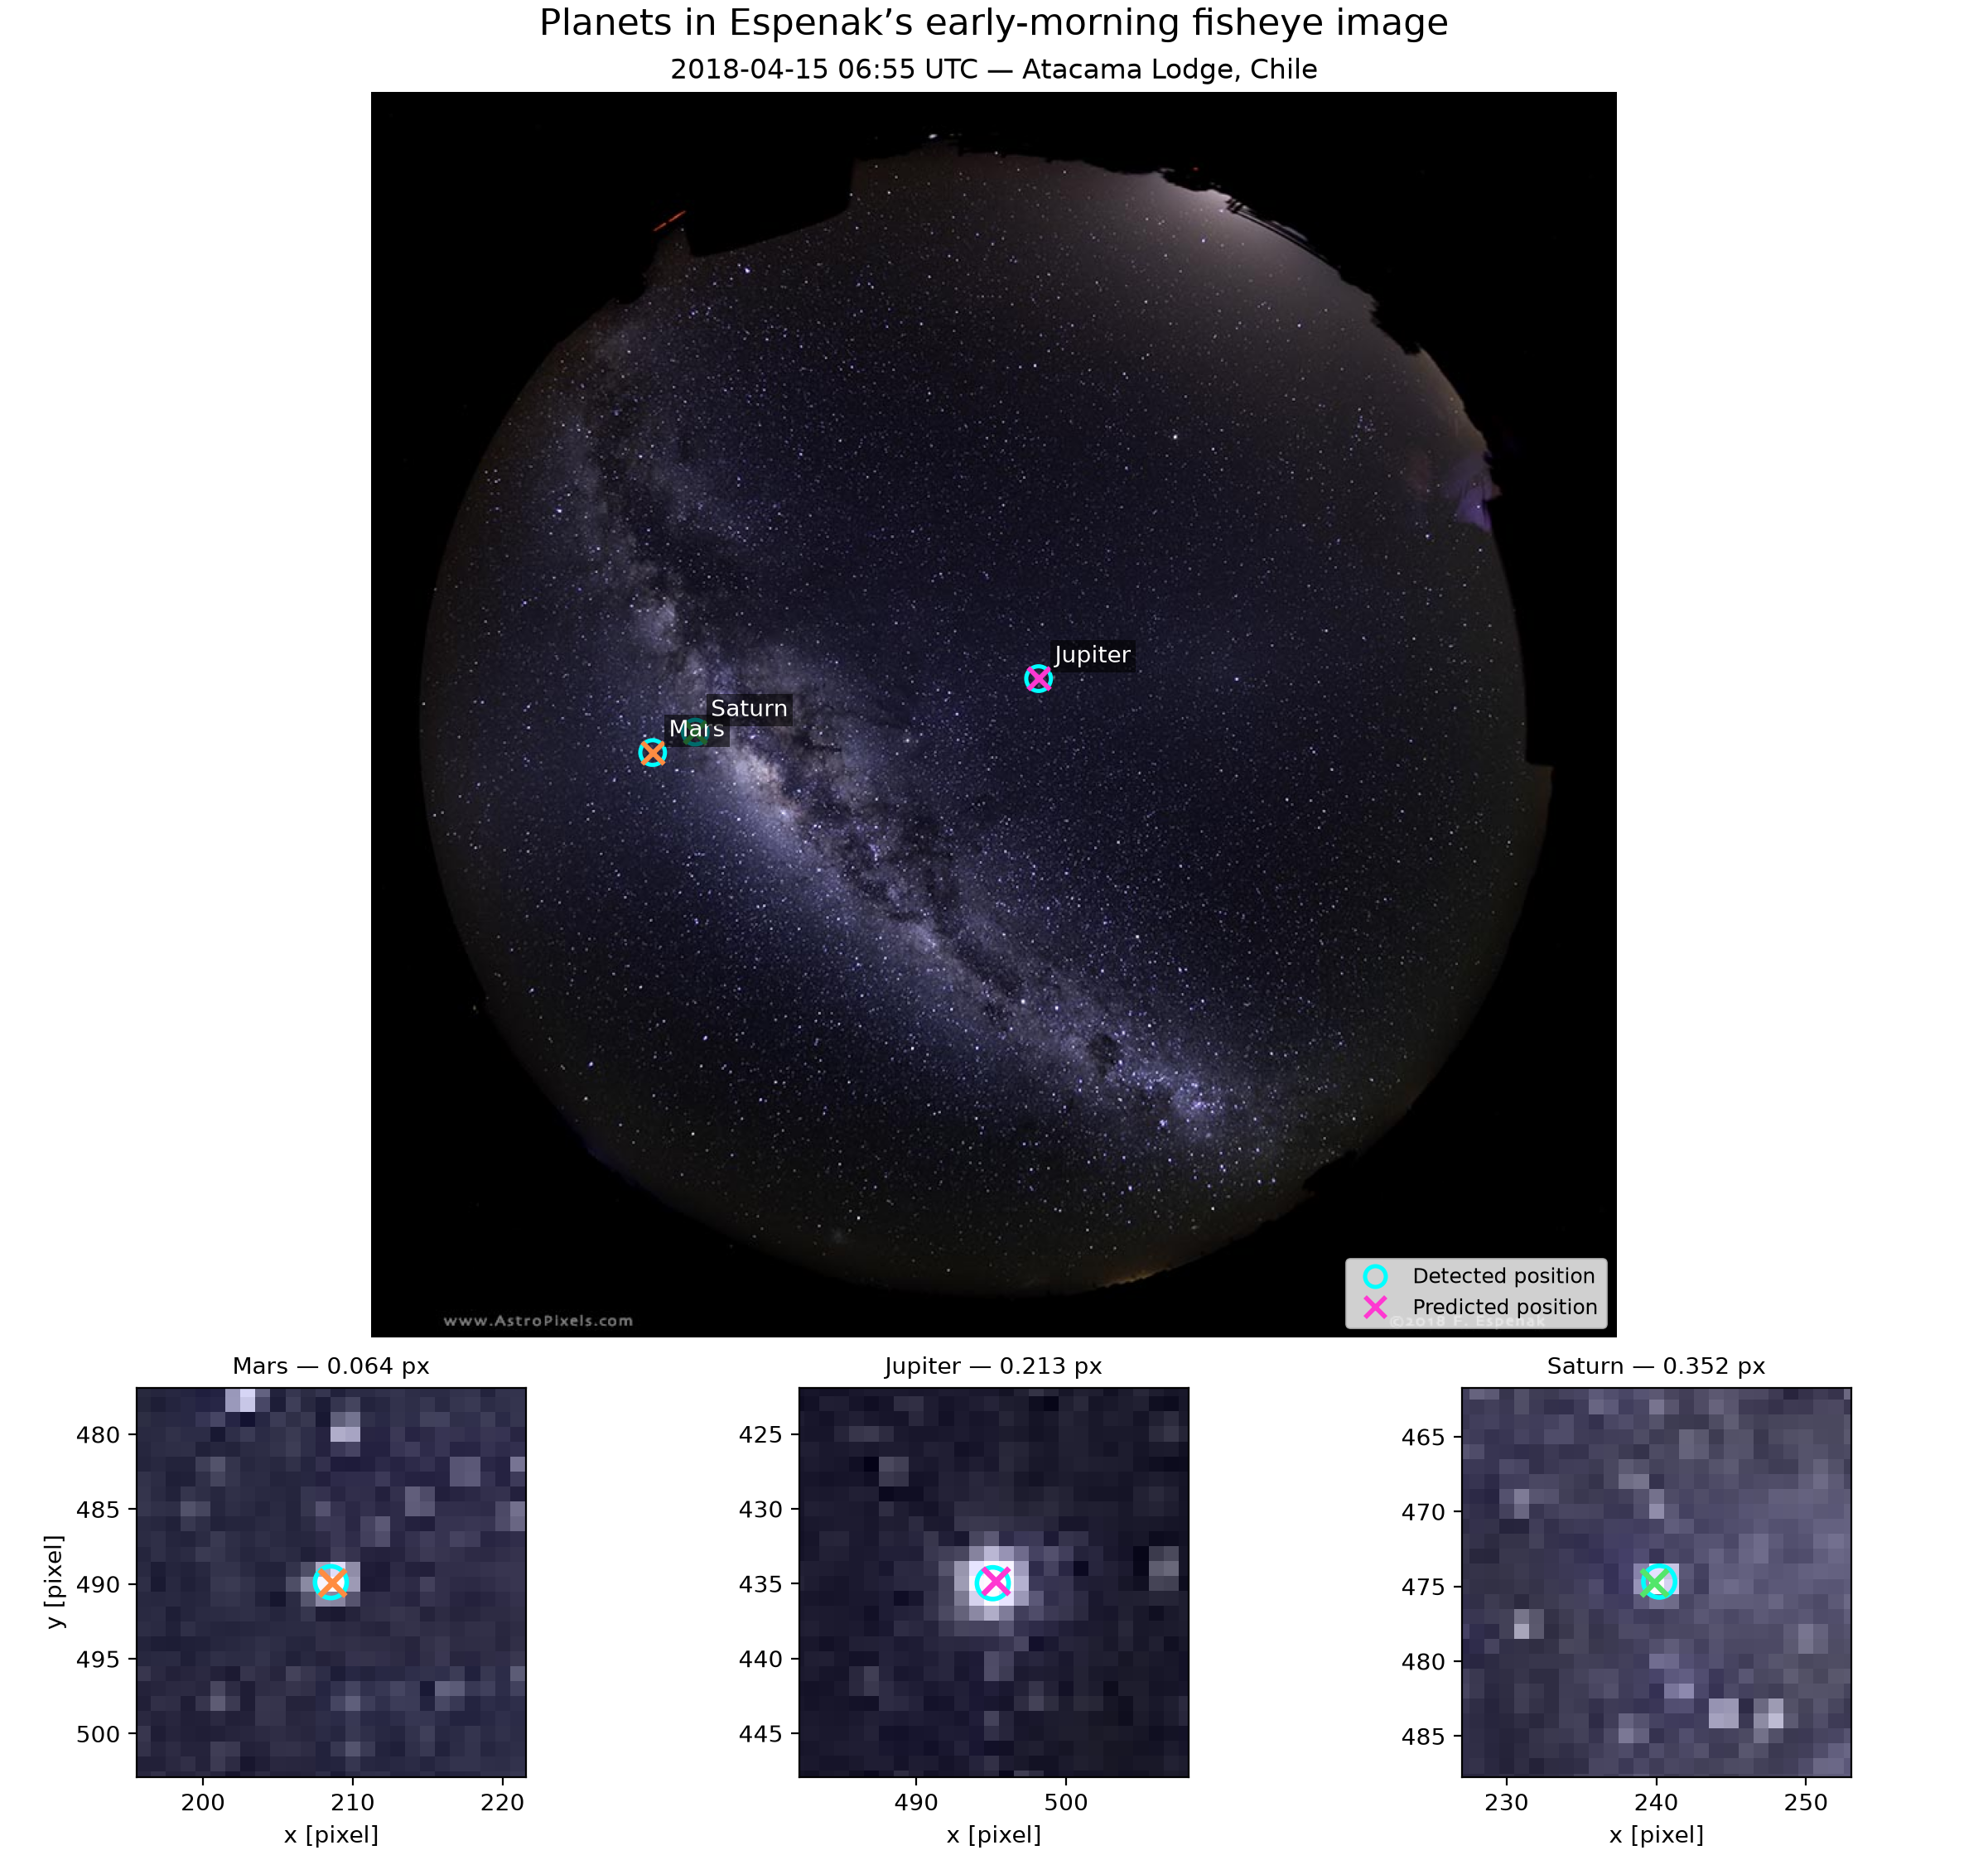
\includegraphics[width=0.88\textwidth]{planet_measured_vs_predicted_overlay.png}
  \caption{Espenak's fisheye image with the three recovered planets. Cyan
  circles show the measured source centroids; coloured crosses show the
  topocentric ephemeris positions projected through the fitted camera model at
  the published epoch. The lower panels show the same coordinates at native
  pixel scale.}
  \label{fig:overlay}
\end{figure*}

\section{Method}
\label{sec:method}

\subsection{Source association and global camera model}

Point sources were detected after local background subtraction. Growing
measurement windows retained broad and saturated sources. We obtained a small
initial constellation with \texttt{tetra3}, ESA's open-source Python
astrometric plate solver for star trackers \citep{tetra3}. Its
``lost-in-space'' pattern matching identifies stars and determines the camera
pointing in right ascension and declination without an initial pointing
estimate. It therefore removes the need for a user-supplied initial sky
pointing or WCS in our workflow, while its solution initialises the subsequent
Barghini-model fit. This does not remove all prior information: tetra3 requires
an approximate field-of-view range and a compatible pattern database. Its
distributed default database covers fields of view from $10^\circ$ to
$30^\circ$ and stars down to magnitude~7 \citep{tetra3}.

Progressive nearest-neighbour association then expanded the solution over the
complete circular field. Every detected source remained available for
association. No catalogue identifier or saved solution was used to seed this
demonstration.

The global projection is the eight-parameter model of
\citet{Barghini2019}, expressed with independent detector positions for the
optical centre $O=(x_O,y_O)$ and reference direction $Z=(x_Z,y_Z)$. For a
detector radius $r_O$ about $O$, the projection angle $u$ is
\begin{equation}
  u(r_O)=V r_O+S\left[\exp(D r_O)-1\right].
  \label{eq:radial}
\end{equation}
The remaining parameter $a_0$ fixes the azimuthal orientation. The transformation
from $(u,b)$ about the optical axis to a celestial unit vector follows the
spherical rotation in Eqs.~(5), (6), and (11) of \citet{Barghini2019}. We fit
the eight parameters by minimising detector-plane residuals between measured
centroids and catalogue directions projected into the image. In the present
celestial solution $Z$ is a fixed bootstrap reference direction; it should not
be interpreted as a fitted terrestrial zenith.

The catalogue-to-camera fit is independent of the manufacturer's nominal
fisheye projection. Its radial mapping, optical centre, and orientation are
therefore inferred from stars. Refraction was not included in this first
planetary experiment. This omission is most consequential near the horizon and
is carried into the empirical residuals rather than corrected cosmetically.

\subsection{Native-plane and repeated photometry}

Instrumental flux is measured independently in each native FITS plane.
Aperture and local-annulus statistics accompany centroid, peak value,
valid-pixel count, and saturation flags. For saturated sources, the clipped
core is excluded and unsaturated wings are retained when sufficient support
remains. Such measurements can support position and a wing-based flux
diagnostic, but are not treated as unsaturated total fluxes.

Catalogue colours provide a basis for instrumental colour terms, while
airmass-like gradients test extinction. Both are diagnostics, not assumptions
used to force the astrometric result. A photometric zenith is reported only
when its likelihood surface has a bounded, informative optimum. It is never
replaced by an airmass field calculated from header site or time.

For repeated images, measurements are joined by fitted catalogue identity
after each exposure has been solved independently. Per-exposure common-mode
offsets are estimated from a stable ensemble, yielding differential light
curves and a scatter--magnitude relation. Quality cuts operate on recorded
flags and measurement support rather than on a preferred light-curve shape.

\subsection{Planetary evidence and the metadata boundary}

After the stellar solution is fixed, unmatched bright detections may be
compared with ephemeris positions. A comparison using the site and time from a
FITS header validates astrometry and metadata jointly; it does not infer the
epoch blindly. A date search can withhold time while supplying a site, as in
the Espenak experiment, but its topocentric likelihood remains conditional on
that site.

\subsubsection{Date search and continuous refinement}

The image positions of all detections were inverted through the fitted camera
model to celestial unit vectors. We evaluated topocentric apparent positions
of Mercury, Venus, Mars, Jupiter, Saturn, Uranus, and Neptune using Astropy's
solar-system transformations \citep{Astropy2022}, whose built-in planetary
model is based on the conventional analytical elements of \citet{Simon1994}.
The stated observing site was used for this topocentric step; geographical
position was not fitted in the experiment reported here.

For every day from 1950 January 1 through 2026 December 31, we found the best
assignment of two different planets to two different initially unmatched
sources and recorded
\begin{equation}
  Q_2(t)=\left[\frac{1}{2}\sum_{p=1}^{2}
       \Delta\theta_p(t)^2\right]^{1/2},
  \label{eq:q2}
\end{equation}
where $\Delta\theta_p$ is the great-circle distance between a measured source
and a planet. Restricting the blind stage to distinct source--planet pairs
prevents a single bright object from satisfying both assignments. At the best
day we again searched \emph{all} detections, rather than preserving the
unmatched classification, and accepted unique associations within
$0.25^\circ$. This recovered a third planet. Holding those three associations
fixed, we minimised the analogous three-planet RMS $Q_3(t)$ continuously within
$\pm2$ d of the daily solution.

This staged procedure separates discovery from precision. The daily search
asks whether the planetary configuration supplies a distinctive calendar date;
the continuous fit measures where the astrometric residual is smallest on that
date. To probe sensitivity to camera-model errors, we drew 2000 sets of three
two-dimensional residual vectors from the fitted stellar residuals, added them
to the planetary centroids, and repeated the fine timing search. This is an
empirical perturbation test, not a formal confidence interval: it neglects
correlated distortion, catalogue systematics, refraction, and uncertainty in
the site.

\section{Results}
\label{sec:results}

\subsection{Stellar and lens solution}

The image yielded 1255 detections, of which 1213 were associated with catalogue
stars; 42 remained unmatched and none was withheld. The camera fit has an RMS
residual of $0.576\px$, a median of $0.367\px$, and a 90th percentile of
$0.745\px$. The fitted optical centre is $(463.79,460.84)\px$. The radial
coefficients are $V=0.00310691$ rad px$^{-1}$, $S=0.00710973$ rad, and
$D=0.00764440$ px$^{-1}$. The implied $90^\circ$ radius is $441.17\px$, and
the central derivative of Eq.~(\ref{eq:radial}) is
$0.18113^\circ$ px$^{-1}$.

At the original $4016$-pixel sampling, the fitted horizon radius would be about
1915 pixels under uniform rescaling, giving a 3830-pixel image circle. This is
consistent with a circular fisheye nearly filling Espenak's square frame. The
agreement is a physical cross-check on the published Nikon D750 and 8-mm Sigma
description; the fit itself used neither camera nor lens metadata. The left
panel of Fig.~\ref{fig:lensdate} also shows that the fitted mapping is not
exactly equidistant, illustrating why the catalogue-derived lens model is
needed for the planetary comparison.

\begin{figure*}
  \centering
  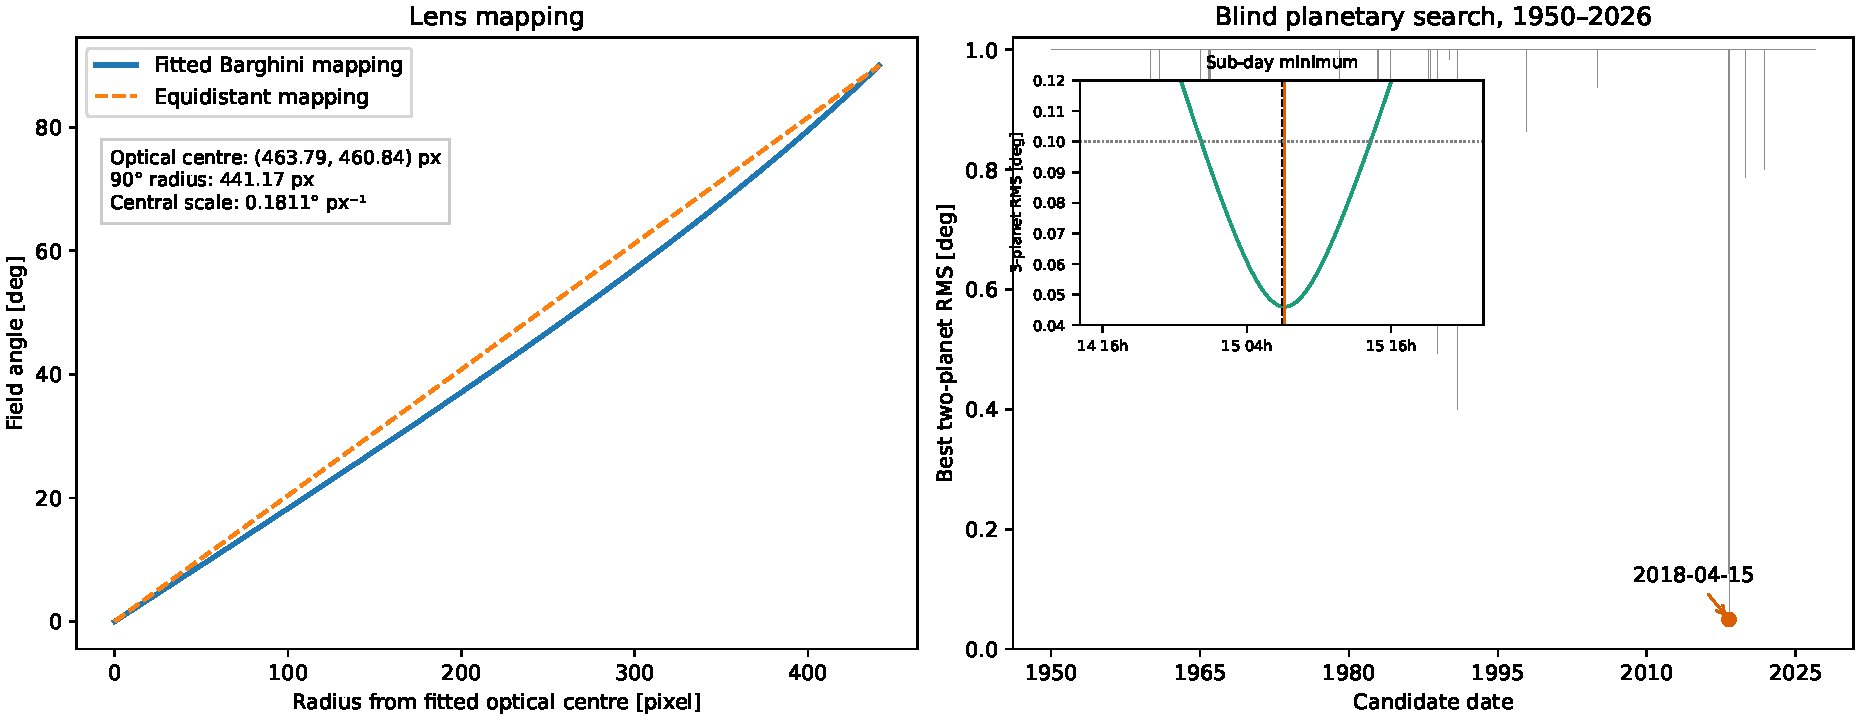
\includegraphics[width=\textwidth]{lens_and_epoch_solution.pdf}
  \caption{Left: fitted Barghini radial mapping and an equidistant mapping with
  the same $90^\circ$ radius. Right: the blind two-planet objective over
  1950--2026, clipped at $1^\circ$ for display. The inset gives the continuous
  three-planet objective around the selected date; dashed and orange vertical
  lines mark the published and best-fitting epochs, respectively.}
  \label{fig:lensdate}
\end{figure*}

\subsection{Planetary date and time}

The blind daily minimum occurred on 2018 April 15, the published date. Its
Jupiter and Saturn assignments had a two-planet RMS of $0.0494^\circ$. After
suppressing dates within 45 d of this solution, the next minimum was 1990
December 19 with $0.4002^\circ$ RMS, eight times larger. Only 18 daily trials
over the 77-year interval fell below $0.5^\circ$, so the global minimum is
strongly distinguished.

Reconsidering all sources on the selected date independently recovered Mars,
Jupiter, and Saturn as detections 36, 8, and 54. At the stated time their
detector-plane residuals were 0.064, 0.213, and 0.352 pixels, respectively
(Fig.~\ref{fig:overlay} and Table~\ref{tab:planets}). The other searched planets
were below the local horizon. The fixed-association continuous minimum was
2018 April 15 07:08:16 UTC with $Q_3=0.0460^\circ$, an offset of 13 min 17 s
from the stated 06:55 UTC.

\begin{table}
  \caption{Recovered planets at the published epoch.}
  \label{tab:planets}
  \centering
  \begin{tabular}{lrr}
    \hline\hline
    Planet & Detection & Separation [pixel] \\
    \hline
    Mars    & 36 & 0.064 \\
    Jupiter &  8 & 0.213 \\
    Saturn  & 54 & 0.352 \\
    \hline
  \end{tabular}
\end{table}

The small offset is an accuracy check against external metadata, rather than a
$13$-minute uncertainty. The interval over which $Q_3<0.1^\circ$ is about
14 h. In the empirical residual-vector experiment, the 16th, median, and 84th
percentiles of the fitted-time displacement were $-2.92$, $-0.08$, and
$+3.00$ h. The 240-s exposure introduces a further two-minute convention shift
if the published time refers to an endpoint rather than mid-exposure. Proper
motion did not usefully constrain this recent date: among the 1127 matched stars
with both components, a reference-year scan changed the RMS by only
$9.8\times10^{-6}\px$ between 2009 and 2018.

\subsection{Dense and heterogeneous stellar fields}

The dense Milky Way solution contains 3653 associations and reaches
0.397892 pixels RMS. Figure~\ref{fig:dense} shows that associations cover the
circular field rather than a favourable central patch and displays the
remaining residual structure. The APICAM example extends the same procedure
to 8032 associations with 0.702-pixel (1.912-arcmin) RMS. Independent Subaru
red and green planes yield 159 and 138 fitted associations. These cases show
that the procedure is not tied to one camera, orientation, catalogue density,
or rendered image format.

\begin{figure*}
  \centering
  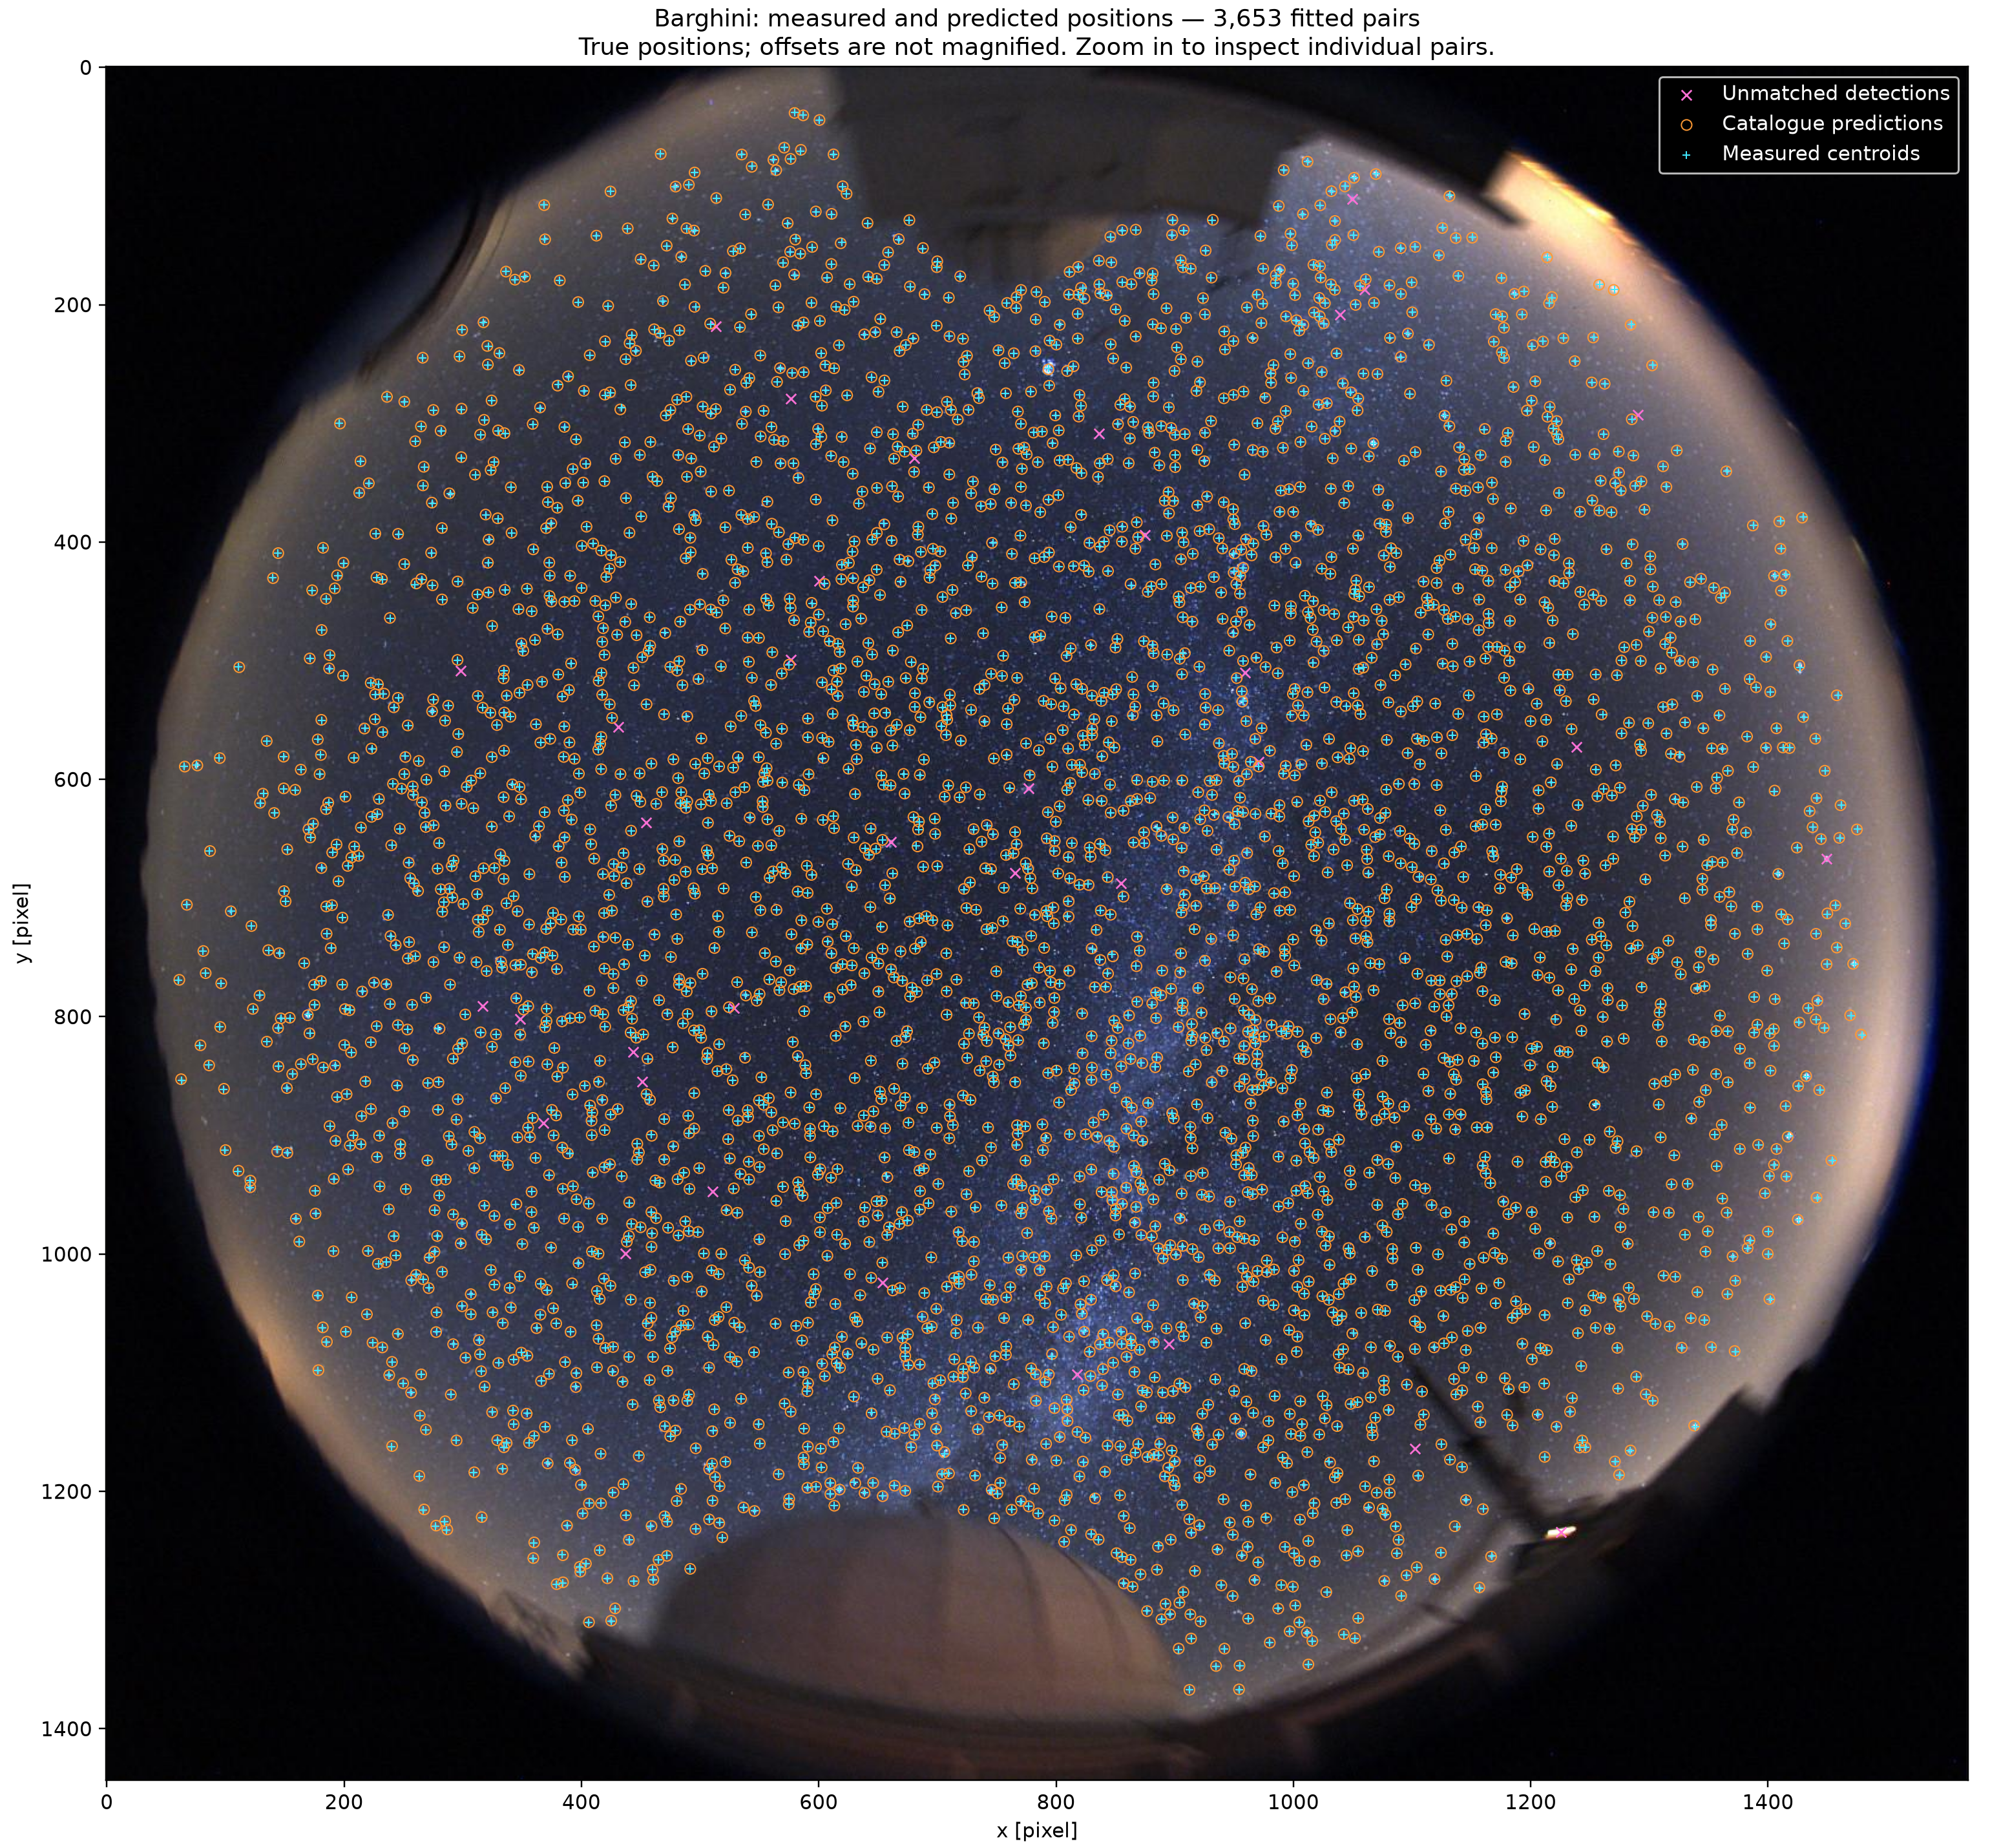
\includegraphics[width=0.49\textwidth]{astrometry_overlay.png}
  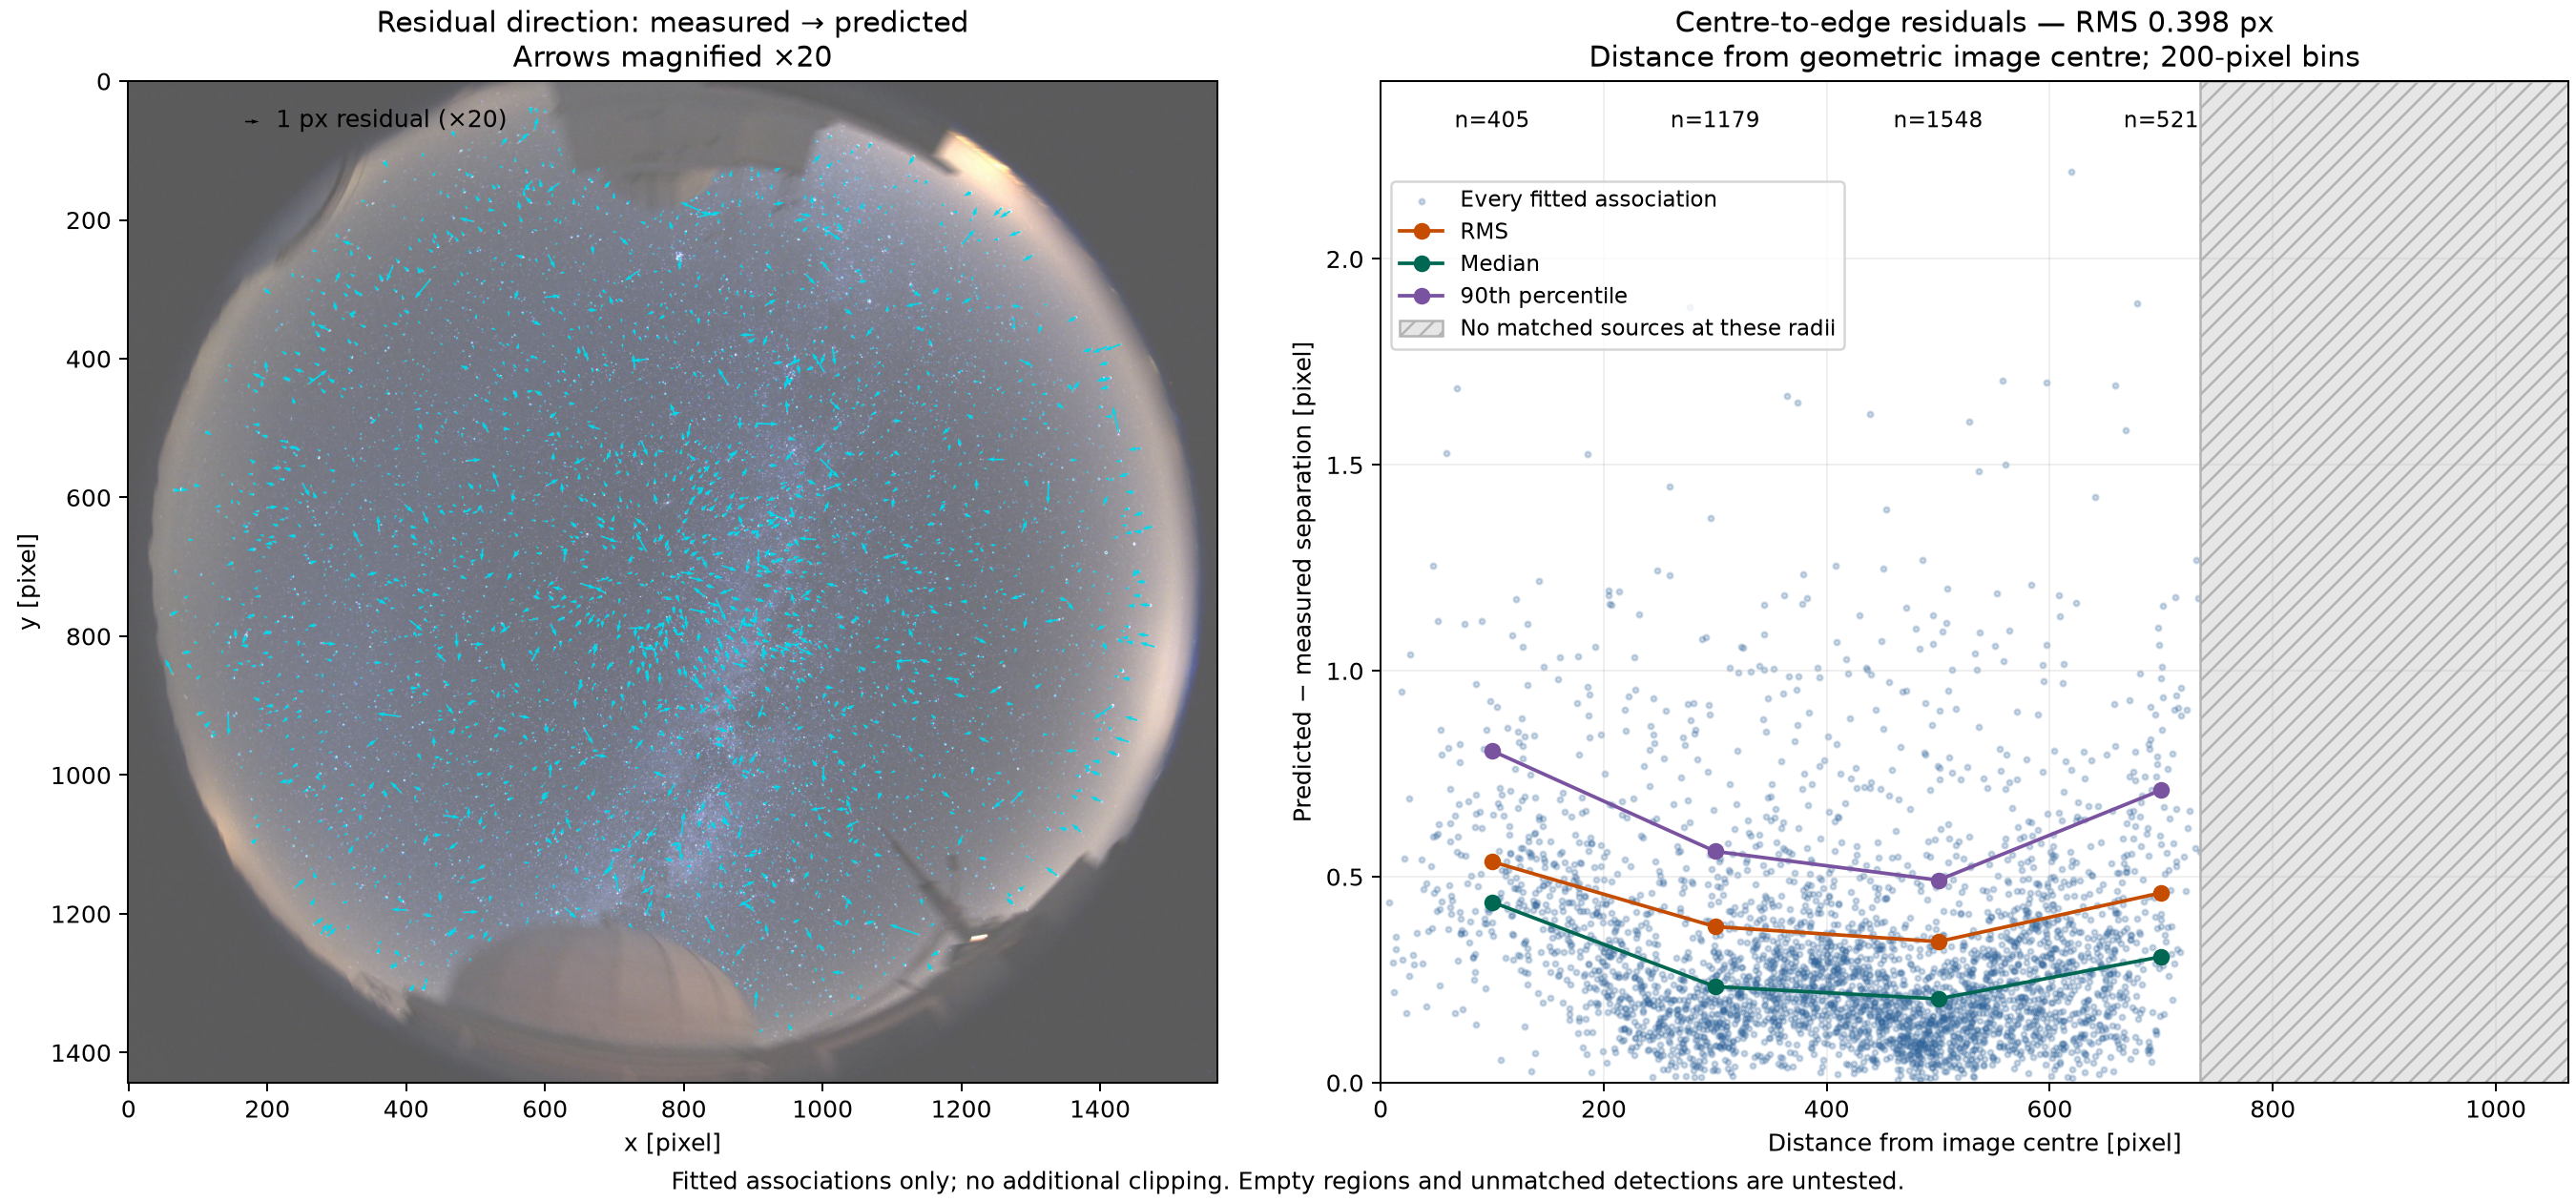
\includegraphics[width=0.49\textwidth]{astrometry_residuals.png}
  \caption{Dense-field solution. Left: measured centroids and catalogue
  predictions across the usable footprint. Right: spatial and distributional
  residual diagnostics. The overlay uses actual coordinates; symbols are not
  shifted radially for visual agreement. Any labelled vector enlargement is
  for legibility only and does not alter numerical residuals.}
  \label{fig:dense}
\end{figure*}

\subsection{A native-colour MMTO exposure}

The representative MMTO frame contains 1512 detections, of which 1385 enter
the final stellar fit. Its 0.337582-pixel RMS corresponds to 2.61083 arcmin;
the median and 90th-percentile angular residuals are 1.738 and 4.149 arcmin.
Figure~\ref{fig:mmto-astrometry} shows both coverage and the residual field,
with measured centroids and predictions plotted at their actual positions.

Neither a stellar catalogue epoch nor a photometric zenith is identifiable in
this exposure. Reporting these negative results prevents a weak profile from
being mistaken for an image-derived date or zenith. Once the blind stellar fit
is fixed, the FITS time identifies Jupiter 0.218247 pixels from detection 1.
Its core is saturated in all three planes, but 372 red, 366 green, and 372
blue wing pixels remain usable. This illustrates why large detections should
be retained and native planes preserved.

\begin{table}
  \caption{Representative astrometric results.}
  \label{tab:wide-results}
  \centering
  \begin{tabular}{lrrr}
  \hline\hline
  Data set & Fitted stars & RMS [px] & RMS [arcmin] \\
  \hline
  Milky Way & 3653 & 0.398 & --- \\
  APICAM & 8032 & 0.702 & 1.912 \\
  Subaru R/G & 159/138 & --- & --- \\
  MMTO & 1385 & 0.338 & 2.611 \\
  \hline
  \end{tabular}
\end{table}

\begin{figure*}
  \centering
  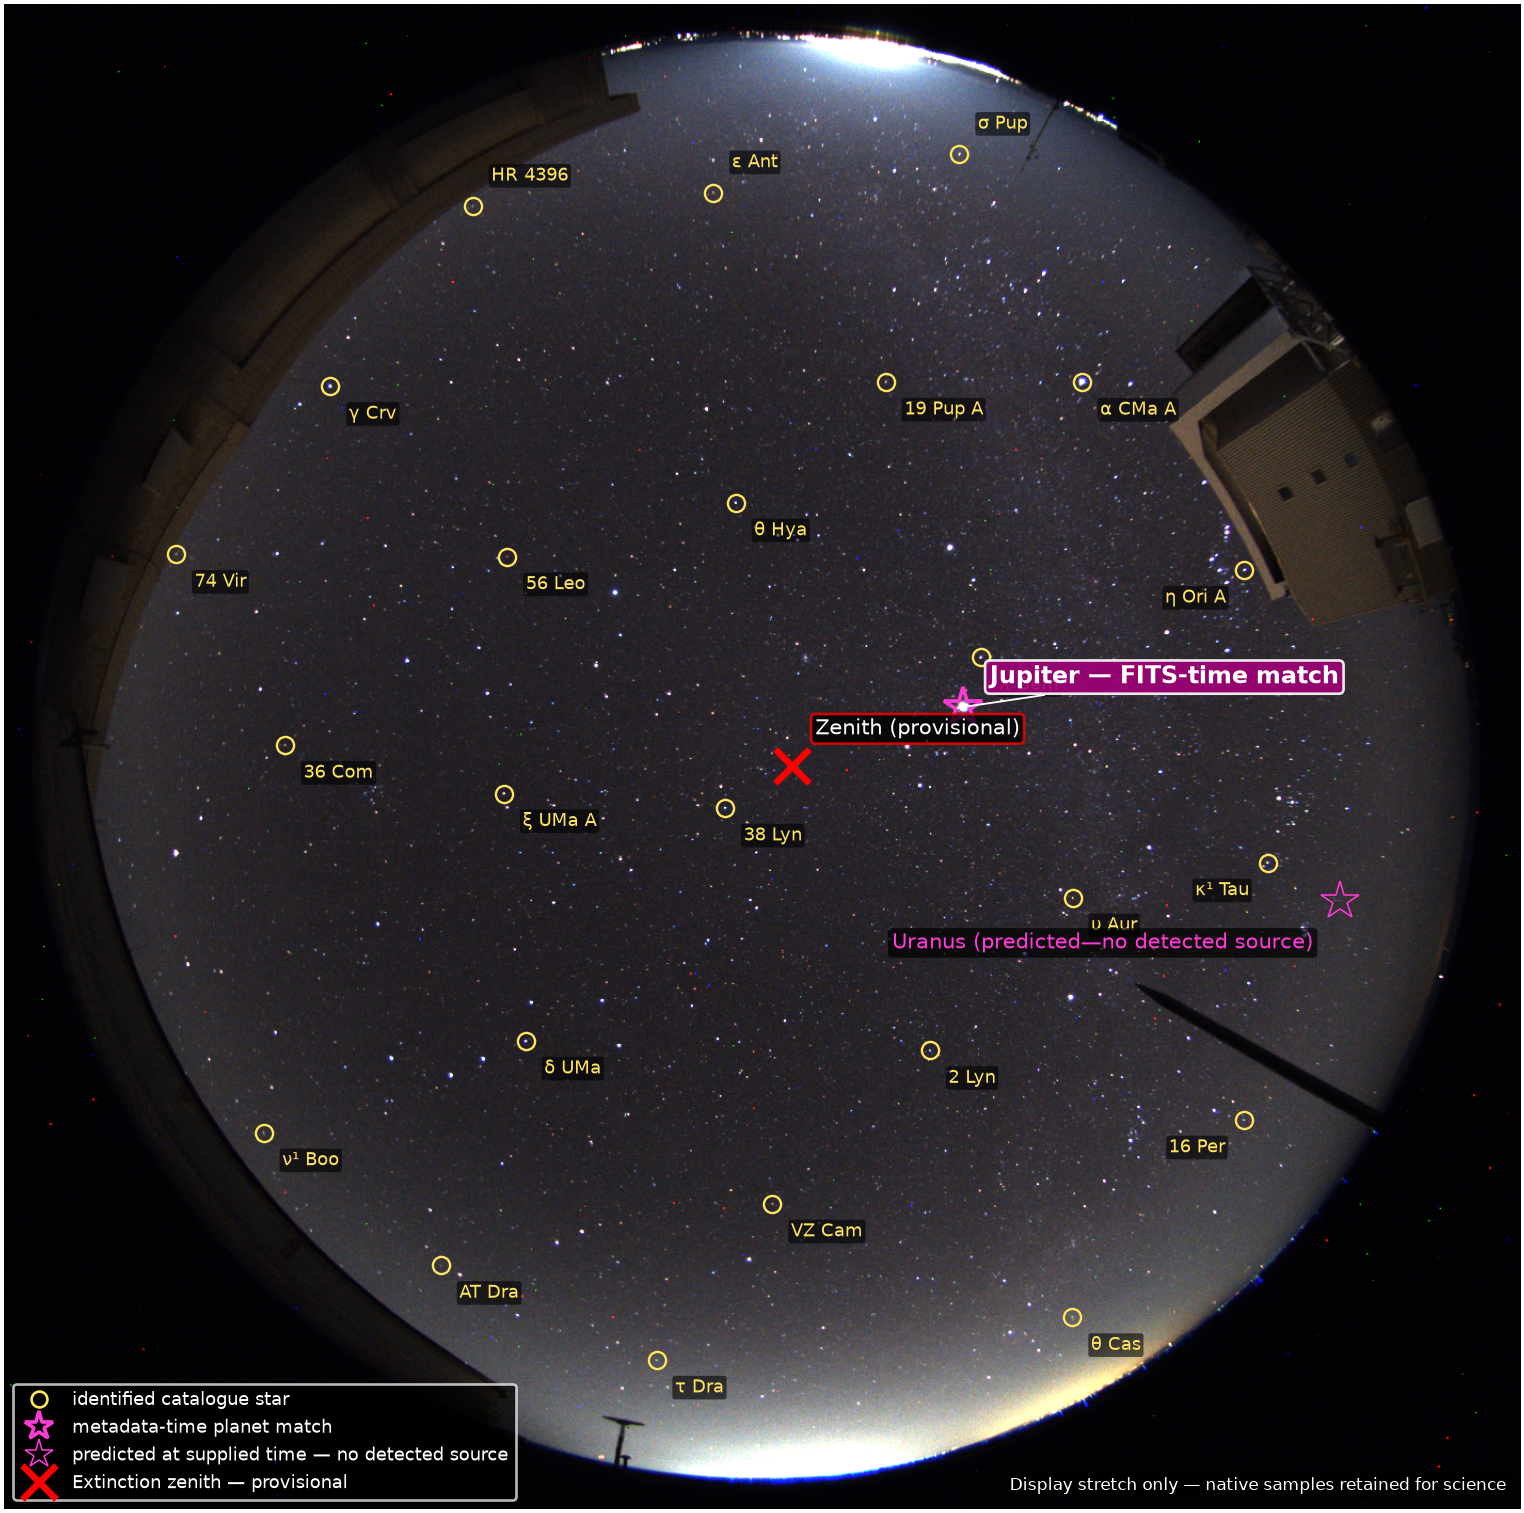
\includegraphics[width=0.49\textwidth]{mmto_sky_overlay.png}
  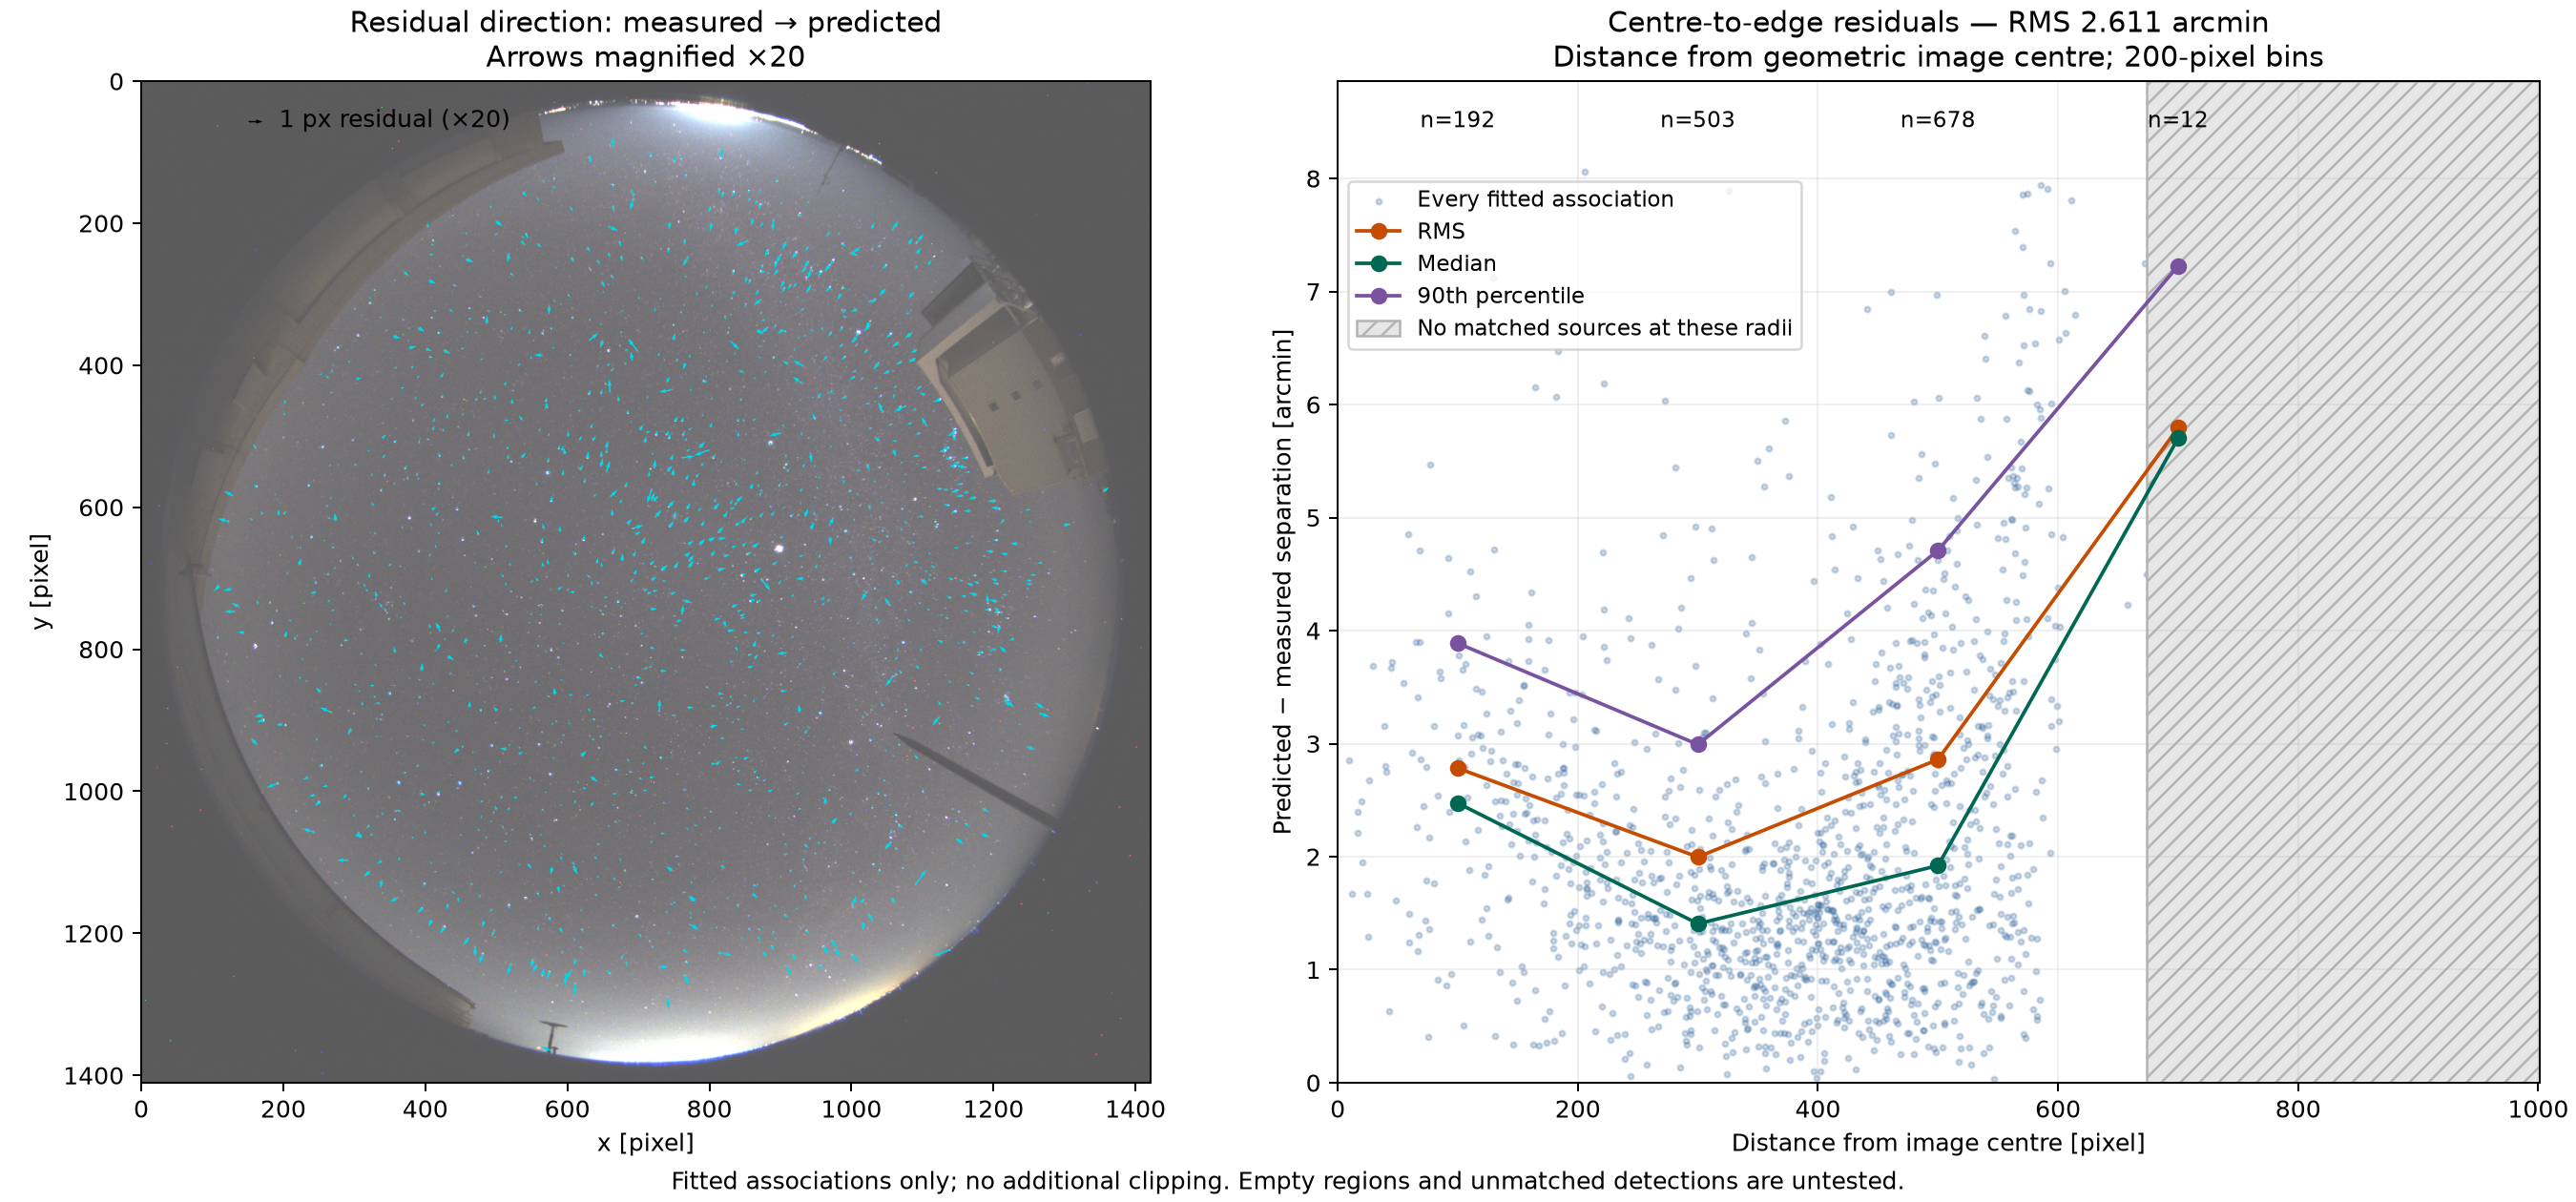
\includegraphics[width=0.49\textwidth]{mmto_astrometry_residuals.png}
  \caption{Representative MMTO exposure. Left: fitted stellar associations
  across the detector. Right: residual diagnostics for 1385 stars. The fit
  has 0.338-pixel (2.61-arcmin) RMS residual.}
  \label{fig:mmto-astrometry}
\end{figure*}

\begin{figure*}
  \centering
  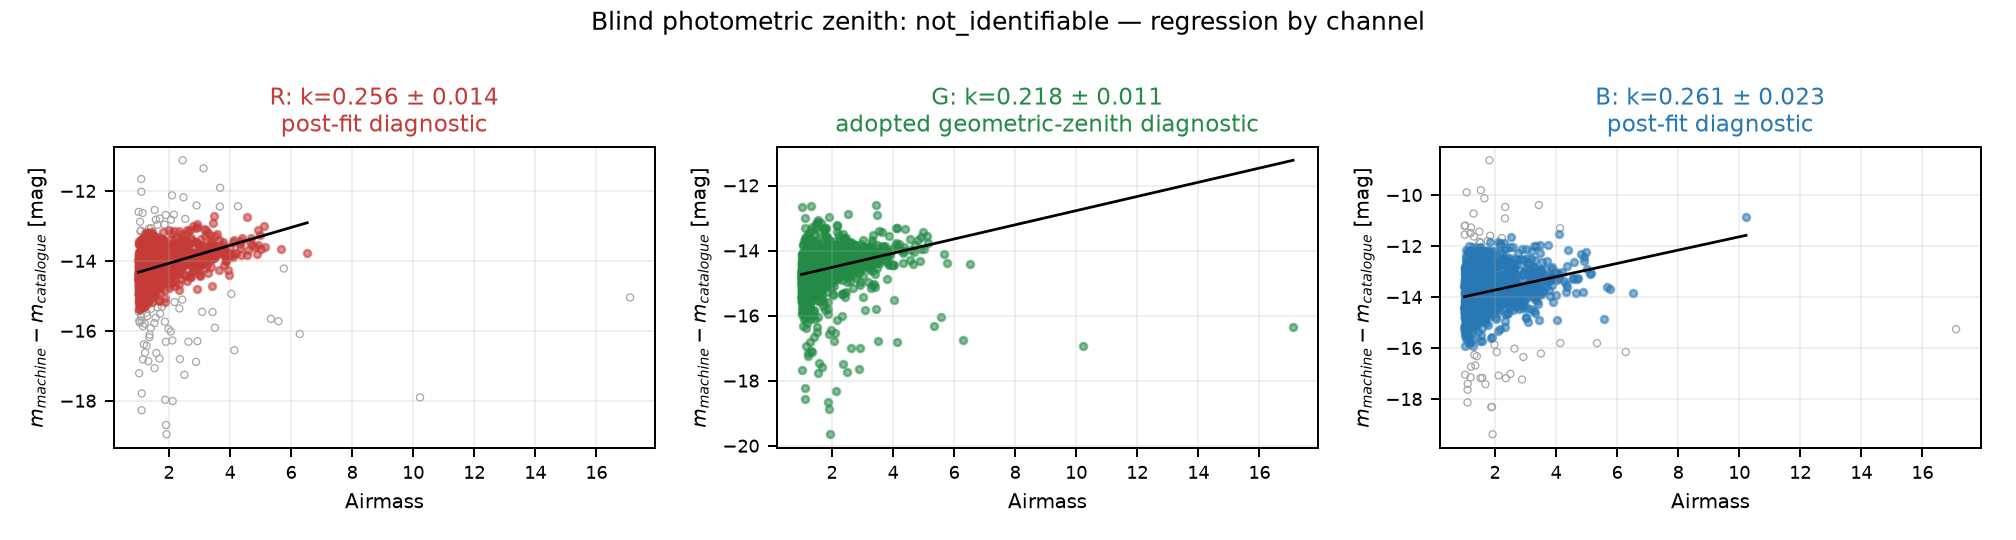
\includegraphics[width=0.49\textwidth]{mmto_extinction_fit.png}
  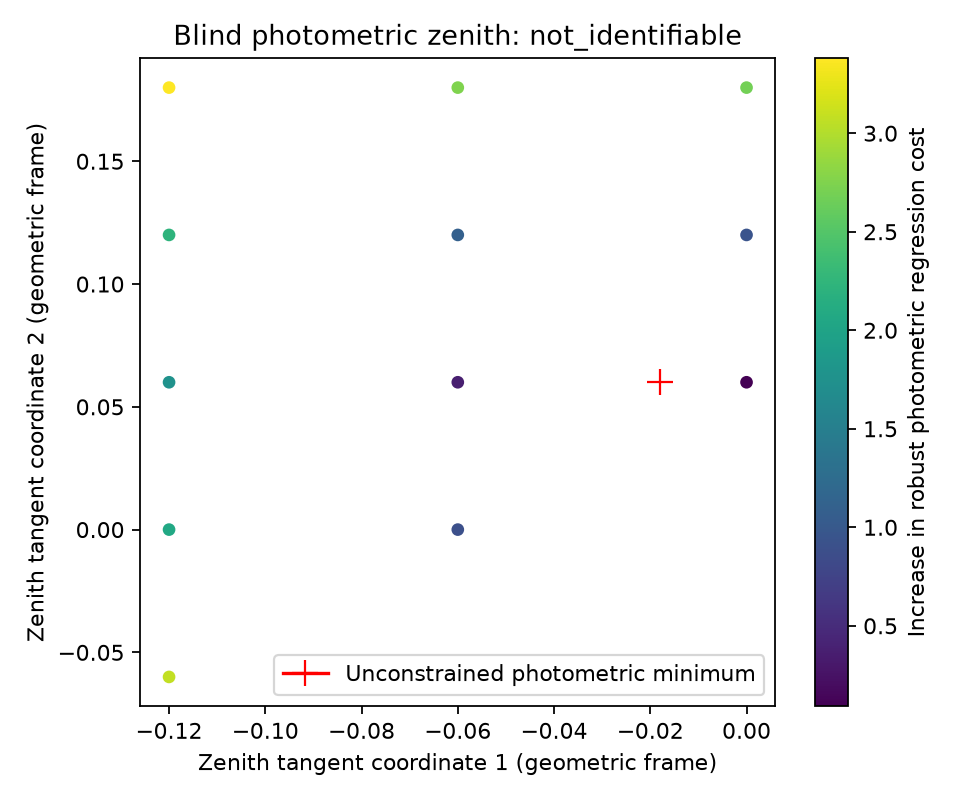
\includegraphics[width=0.49\textwidth]{mmto_zenith_profile.png}
  \caption{Photometric diagnostics for the same exposure. The colour and
  extinction regression (left) is measurable, but the profile (right) does
  not identify a photometric zenith. It is reported as a non-detection, not
  replaced by a metadata-derived airmass centre.}
  \label{fig:mmto-photometry}
\end{figure*}

\subsection{Repeated MMTO photometry}

The repeated product contains 66 solved runs. One duplicate is omitted,
leaving 65 exposures. Of 86\,423 input measurement rows, 152 fail recorded
quality criteria and 86\,271 remain. Ensemble correction produces 162
green-plane stellar time series. The light curves in
Fig.~\ref{fig:mmto-lightcurves} retain shared temporal structure and
star-to-star differences; they were not selected to resemble a predetermined
variability pattern. Figure~\ref{fig:mmto-scatter} gives the corresponding
precision envelope and exposes objects whose variability or measurement
problems exceed the stellar locus.

\begin{figure*}
  \centering
  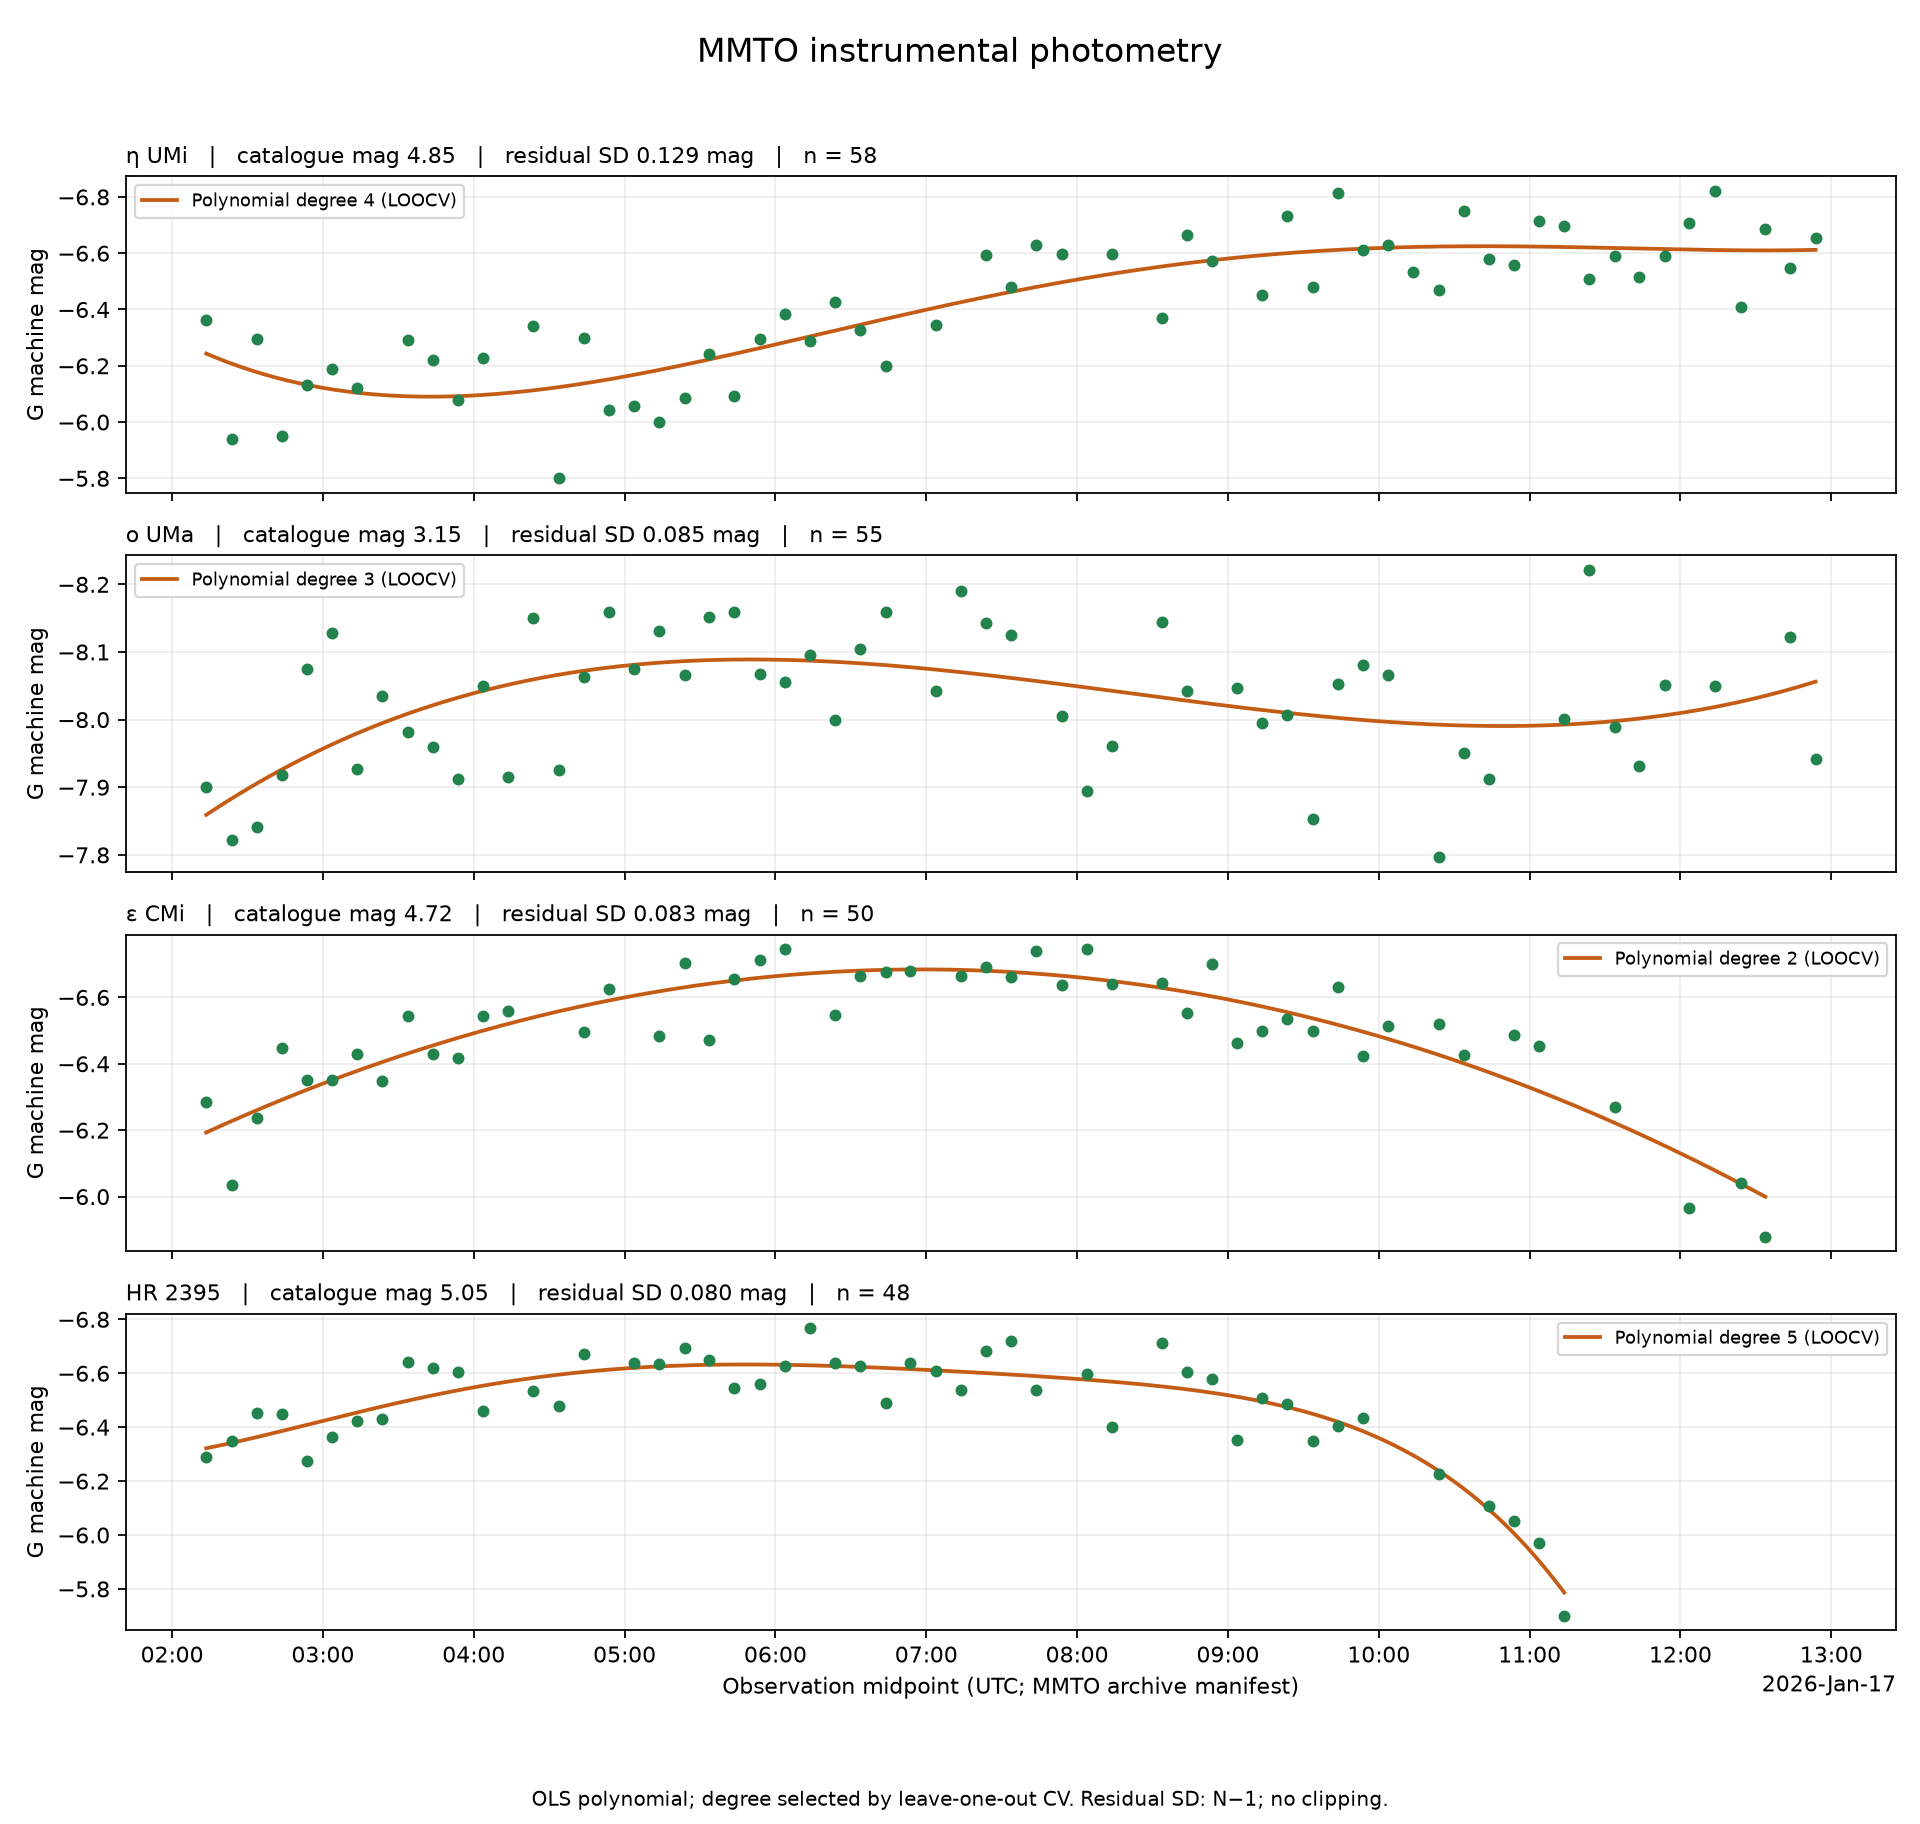
\includegraphics[width=0.96\textwidth]{mmto_lightcurves.png}
  \caption{Differential green-plane light curves from 65 MMTO exposures.
  Catalogue identity links measurements only after each exposure's independent
  astrometric solution. The collection contains 86\,271 usable measurements
  in 162 stellar series.}
  \label{fig:mmto-lightcurves}
\end{figure*}

\begin{figure}
  \centering
  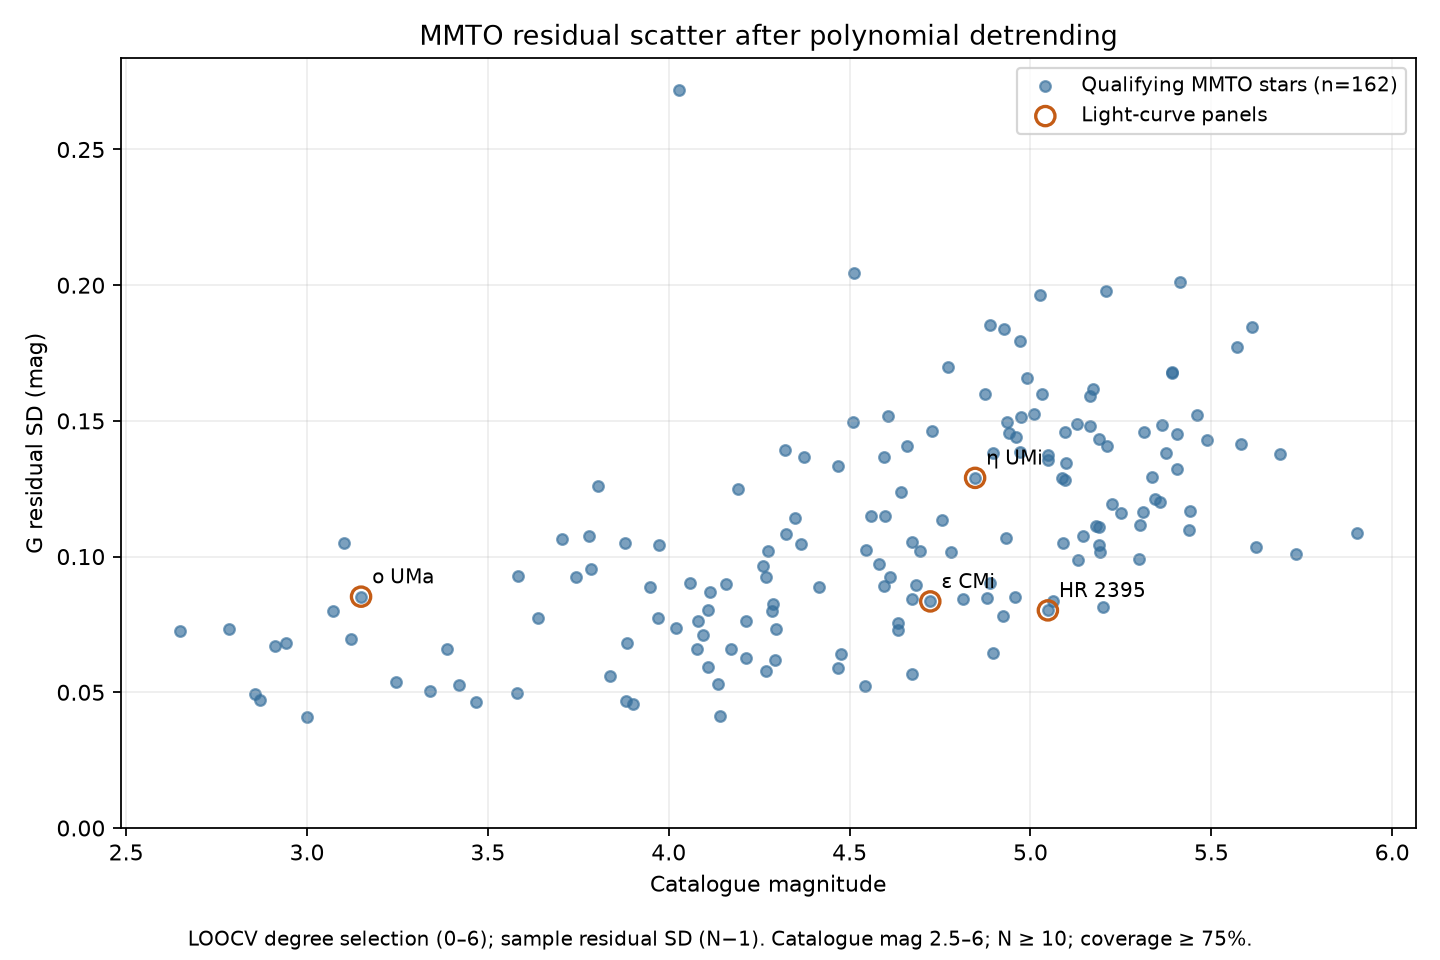
\includegraphics[width=\columnwidth]{mmto_scatter_vs_magnitude.png}
  \caption{Time-series scatter versus instrumental magnitude. The lower locus
  describes achieved repeatability; objects above it warrant astrophysical or
  measurement-level inspection.}
  \label{fig:mmto-scatter}
\end{figure}

\section{Why native-colour repeated archives matter}
\label{sec:archives}

A rendered RGB image is useful for inspection but is a lossy scientific
product. White balance, gamma, clipping, compression, and resampling mix or
discard quantities needed to compare detector response with catalogue colour.
A repository of native-colour FITS images retains four capabilities that
cannot reliably be reconstructed later.

First, separate red, green, and blue values permit instrumental colour terms
and colour-dependent extinction to be measured rather than guessed. Second,
linear values and saturation masks allow usable wings to be separated from
clipped cores. Third, headers and explicit valid-pixel support make
calibrations and exclusions auditable. Fourth, repeated frames turn isolated
measurements into ensembles: common transparency changes can be removed,
repeatability quantified with magnitude, and variability tested against
neighbouring stars.

The MMTO results make the gain concrete. One frame supports a 1385-star
solution, a three-colour extinction diagnostic, and a saturated-wing planetary
validation. The repeated archive supports more than 86\,000 controlled
measurements and 162 light curves. A preview retains the visual scene but
forfeits much of this evidence. A useful repository should preserve original
planes, checksums, timestamps, calibration context, and per-exposure
provenance alongside rendered products.

\section{Discussion}
\label{sec:perspectives}

Dating a single sky image to the correct day is useful wherever provenance is
The strongest result is the common measurement chain: blind initialization,
dense global astrometry, native-plane photometry, and optional post-fit
physical diagnostics. Its outputs remain separable. A good stellar solution
does not guarantee that catalogue epoch, zenith, or observing time is encoded
strongly enough to measure; conversely, a saturated planet can provide a
precise positional validation when its wings are preserved.

Residual maps are essential because one RMS value compresses field-dependent
distortion, centroid bias, refraction, and catalogue mismatch. Future work
should propagate centroid uncertainty, colour-dependent refraction, exposure
duration, and camera-parameter covariance into a joint sky-coordinate
likelihood. The present light curves are differential instrumental
measurements, not standard-system magnitudes; dedicated flat-field,
non-linearity, and colour calibration remain necessary.

incomplete: digitised plate and film collections, meteor and auroral archives,
environmental all-sky cameras, and historical or public astrophotography. Large
photographic archives already open century-long time baselines
\citep{Grindlay2009}; an astronomical timestamp can expose catalogue mistakes,
order undated sequences, and connect an image to observing logs or transient
events. In particular, a date recovered for a historical image containing a
nova could place that observation on the nova light curve and constrain its
rise, peak, or decline. This is valuable for epochs before systematic patrol
cameras supplied dense time-series coverage. A planetary solution is also
independent of file timestamps and many camera-clock failures.

The 13-minute agreement in this example is interesting because it comes from
the celestial scene in one static exposure, but it should be understood as a
target for a coupled model. Planetary angular velocities near the observed
configuration convert small astrometric biases into hours of timing shift. A
fit that simultaneously includes a physical zenith, latitude, atmospheric
refraction and extinction, camera geometry, and the finite exposure should
separate these effects. Star-trail angular length can supply exposure duration;
the distribution of photometric residual against airmass can constrain the
zenith and extinction; and the resulting terrestrial orientation can supply
local sidereal time. Together these observables could turn the sharp formal
planetary minimum into a defensible sub-hour uncertainty and might constrain an
unknown observing latitude as well as the epoch. Testing that prospect requires
multiple images, deliberately blinded metadata, and injected perturbations.

\section{Conclusions}

Blind initialization followed by Barghini-model refinement fits thousands of
stars across strongly distorted fields without cached identities or
metadata-seeded pointing. Retaining every detection permits bright-object
astrometry and wing measurements that early rejection would lose. Native red,
green, and blue FITS planes support auditable colour and extinction
diagnostics, while repeated frames support differential light curves and
empirical precision estimates.

Planet matches, catalogue epoch, and photometric zenith remain conditional
measurements. They must be reported with their metadata boundary and
identifiability, including explicit non-detections. The Espenak experiment
recovers a calendar date conditional on a supplied site, but its formal
13-minute offset does not supersede its several-hour empirical sensitivity.

Repositories of repeated, native-colour FITS observations are therefore
scientific infrastructure rather than image galleries. They preserve the
information needed to recalibrate, validate, and extend measurements long
after a rendered preview has exhausted its scientific use.

\begin{acknowledgements}
We thank Fred Espenak for publishing the image and its observing metadata. The
image remains credited to and copyrighted by its photographer; its use here is
for scientific analysis. This work made use of Astropy and tetra3.
\end{acknowledgements}

\section*{Data and code availability}
The figure-generation code, numerical summaries, and verification tests
accompany the solver and manuscript repositories. Figure source paths, run
identifiers, SHA-256 checksums, numerical claims, and interpretive caveats are
recorded in \texttt{data/figure\_provenance.json}. The exact pre-revision
manuscript is retained in
\texttt{archive/2026-09-18-pre-revision/}. The Espenak input is available from
the publisher's page, subject to the photographer's terms
\citep{Espenak2018}; the MMTO native FITS archive remains under its repository
access terms.

\bibliographystyle{aa}
\bibliography{references}
\end{document}
